\chapter{Introduzione}
\label{chap:intro}
\vspace{1cm}
Questo capitolo fornisce un'introduzione agli argomenti trattati nel corso di questa
tesi, fornendo le motivazioni per cui si \`e ritenuto necessario svolgere questo
lavoro.

La sezione \ref{sec:introSoC} fornisce una panoramica introduttiva del contesto in cui si
inquadra l'argomento della tesi, illustrando i concetti di \emph{\acl{SoC}} e
\emph{\acl{MPSoC}} e il vantaggio che deriva in termini di rapporto prestazioni/costi.

La sezione \ref{sec:reconfComp} introduce il concetto di \emph{sistemi riconfigurabili},
e mostra come le architetture hardware possono effettivamente beneficiare dell'impiego
di questa tecnica per soddisfare i requisiti di performance; viene inoltre presentata
la struttura di un generico flusso di sviluppo per \acs{MPSoC} riconfigurabili.

La sezione \ref{sec:definizioneProblema} descrive il problema del \emph{mapping} e dello
\emph{scheduling} di un'applicazione su architetture riconfigurabili; particolare
enfasi viene posta sull'importanza che queste fasi rivestono all'interno del
flusso di sviluppo e sul perch\'e questo problema sia impegnativo da risolvere
e tuttora oggetto di ricerca non solamente in ambito informatico.

\newpage

\section[Introduzione a \acs{SoC} e \ac{MPSoC}]{Introduzione a \acs{SoC} e \ac{MPSoC}}
\label{sec:introSoC}
Il continuo aumento delle performance richieste ai sistemi informatici ha portato alla necessit\`a
di trovare nuove soluzioni per aumentare le prestazioni dei processori. Negli ultimi anni si \`e
assistito a un drastico cambiamento del paradigma di computazione, segnato dal progressivo passaggio
dalle architetture single-core a quelle multi-core \cite{SingleCoreToMultiCore}.

La versione semplificata della famosa osservazione empirica enunciata da Gordon Moore, secondo la quale
si assiste a un raddoppio della velocit\`a e delle prestazioni dei processori ogni due anni, non \`e
pi\`u valida: mentre negli anni '70 la frequenza di clock di un processore Intel \`e passata da 108 KHz a
5 MHz, nella prima decade del nuovo millennio essa \`e passata da 1.5 GHz
a 3.8 GHz \cite{IntelTimeline}. Dal 2006 Intel, AMD, IBM e altri produttori hardware non sono riusciti a produrre
processori pi\`u veloci perch\'e il chip subiva un eccessivo surriscaldamento.

Malgrado ci\`o, la versione originale dell'enunciato di Moore \`e ancora valida, e il numero di transistor
all'interno di un processore effettivamente continua a raddoppiare circa ogni due anni, grazie ai continui progressi
nel loro processo di fabbrica \cite{MooreLawPastPresentFuture}. Ad esempio, nel decennio 2000-2009, il numero di transistor all'interno di
un processore \`e passato da 37,5 milioni a 904 milioni, e Haswell, l'ultima microarchitettura Intel
rilasciata nel 2013, \`e ottenuta mediante processo produttivo a 22 nm.
A titolo esemplificativo, la tabella \ref{tab:processoProduttivo} illustra il processo produttivo utilizzato per
alcune architetture rilasciate negli ultimi anni.


Stanti queste premesse, la continua miniaturizzazione dei componenti ha permesso di condensare
un numero sempre maggiore di elementi su un singolo chip, ed \`e stata resa possibile la produzione di
architetture con un numero di core in continuo aumento. Intel ha prototipizzato \emph{Polaris} \cite{IntelPolaris},
un processore contenente 80 core, AMD con la serie Opteron\texttrademark{} 6200 ha commercializzato
un'architettura a 16 core.
Particolare importanza alla luce di questi progressi tecnologici assumono i \ac{MPSoC} \cite{MPSoCBook}, ovvero sistemi
caratterizzati non soltanto da un microprocessore (multi-core, contrariamente ai \ac{SoC} \cite{SoCBook}, caratterizzati
da un processore single-core), ma anche da varie unit\`a funzionali quali
blocchi di memoria, connettori per interfacce USB, FireWire, Ethernet e altre periferiche, collegati
tra loro tramite BUS. Le architetture \ac{MPSoC} si dividono in due categorie \cite{IntroMPSoCTrendsChallenges}:
\begin{itemize}
  \item omogenee, quando gli elementi processanti sono tutti di un unico tipo, ad esempio un processore
    multi-core;
  \item eterogenee, quando gli elementi processanti si differenziano per il loro tipo, ad esempio processori,
    logica riconfigurabile oppure processori dedicati come i \acs{DSP}.
\end{itemize}
 

\begin{table}[t]
  \begin{center}
    \begin{tabular}{|c|c|c|c|}
      \hline
      \textbf{Architettura} & \textbf{Produttore} & \textbf{Anno di rilascio} & \textbf{Processo produttivo}\\
      \hline
      Nehalem & Intel & 2008 & 45 nm\\
      \hline
      Bobcat & AMD & 2011 & 40 nm\\
      \hline
      Bulldozer & AMD & 2011 & 32 nm\\
      \hline
      Sandy Bridge & Intel & 2011 & 32 nm\\
      \hline
      Jaguar & AMD & 2013 & 28 nm\\
      \hline
      Haswell & Intel & 2013 & 22 nm\\
      \hline
    \end{tabular}
    \caption{Processo produttivo di alcune microarchitetture Intel
      \cite{IntelTransistor, IntelsVision} e AMD.}
    \label{tab:processoProduttivo}
  \end{center}
\end{table}



\section{Sistemi riconfigurabili e introduzione ai flussi di sviluppo}
\label{sec:reconfComp}
L'integrazione introdotta nella precedente sezione tuttavia apre una serie di problemi nella progettazione
di un \ac{MPSoC}, tra cui elevato costo di progettazione dei sistemi, bassa affidabilità e, ultimo
ma non meno importante, necessità di controllare il consumo di energia; uno dei metodi che 
permette di risolvere i problemi sopra citati  \`e l'utilizzo dei \emph{sistemi riconfigurabili}.

Con il termine \emph{sistemi riconfigurabili} si intendono delle architetture hardware che 
offrono la possibilità di essere riconfigurate per implementare qualsiasi funzionalità 
l'utente desideri. Elementi computazionali composti da logica riconfigurabile possono essere integrati in un
\ac{MPSoC} \cite{EmbeddedReconfigurableArchitectures}. Le caratteristiche e il fondamento logico alla
base delle architetture riconfigurabili,
oltre ai vantaggi che conseguono dal loro utilizzo sono descritte nelle prossime sezioni.

\subsection{Da von Neumann alle architetture riconfigurabili}
\label{subsec:cambioParadigma}
In questa sezione vengono illustrati i due principali modelli concettuali di architettura
informatica convenzionalmente trattati: il modello \emph{general-purpose} e il modello
\emph{application-specific}. Vengono presentati pregi e difetti di ciascuna architettura
e viene spiegato come i sistemi riconfigurabili cerchino di combinare i vantaggi di
entrambe.

\subsubsection{Il modello general-purpose}
Il modello general-purpose è tuttora ampiamente utilizzato, soprattutto nei personal
computer che utilizziamo tutti i giorni. Questa architettura, proposta dal matematico
John von Neumann nel 1945 \cite{First-Draft-Report-EDVAC}, è basata sul concetto di
\emph{stored-program} computer; la particolarità di uno stored-program computer è quella
di tenere le istruzioni dei programmi e i relativi dati nella memoria RAM. Un calcolatore di
questo tipo contiene una \ac{ISA}\footnote{Il termine \acl{ISA} viene usato per descrivere
una serie di caratteristiche dell'architettura di un computer, ad esempio le istruzioni
a disposizione, i registri, l'architettura della memoria, le modalità di indirizzamento, etc.}
e può memorizzare un programma composto da un insieme di istruzioni che guideranno
la computazione. Contrariamente alle architetture precedenti, che potevano eseguire
solamente un programma preimpostato, il vantaggio dell'architettura general-purpose consiste
nella possibilità di eseguire codice arbitrario.

\subsubsection{Il modello application-specific}
Mentre il modello visto nella sezione precedente consente di avere una maggiore
flessibilità a discapito però delle prestazioni che può fornire, il modello
application-specific si posiziona all'estremo opposto rispetto al primo: è infatti
caratterizzato da elevate prestazioni e da un basso consumo di potenza. Questo modello
computazionale viene realizzato mediante l'impiego di componenti chiamati \acp{ASIC}
\cite{ASICMicroprocessors},
dei circuiti integrati progettati per svolgere un'unica funzionalità. Questo guadagno
in prestazioni comporta tuttavia uno svantaggio in termini di costi di produzione e,
naturalmente, una minore flessibilità.


\subsubsection{I due approcci combinati}
Secondo l'informatico Reiner Hartenstein, le architetture riconfigurabili introducono un
cambio di paradigma rispetto all'architettura di von Neumann
\cite{HartensteinParadigmShift}. In un articolo del 1991, Hartenstein et al.~presentano
una nuova metodologia di design per lo sviluppo rapido di \ac{ASIC} ad alte prestazioni,
partendo da specifiche di algoritmi ad alto livello \cite{HartensteinNovelASICDesign};
questa metodologia è basata su un nuovo paradigma di macchina sequenziale, chiamata da
Hartenstein \emph{anti macchina}\footnote{Così definita per le sue differenze rispetto al
più convenzionale modello di von Neumann.} o \emph{Xputer} \cite{HartensteinNovelASICDesign}.\footnote{Il termine
\emph{Xputer} ha origine dalla necessità dei suoi ideatori di rimpiazzare le prime tre
lettere della parola ``computer'' con un altro prefisso. Non trovandone uno, è stato
deciso che queste lettere fossero rimpiazzate dalla lettera ``x''.}

La principale caratteristica che la differenzia rispetto all'architettura di von Neumann è
l'essere guidata da flussi di dati (data-streams) piuttosto che da flussi di istruzioni
(instruction-streams), idea alla base degli \emph{array sistolici}
\cite{SystolicArraysConceptImplementation}.\footnote{Negli array
sistolici la computazione è affidata a una matrice di \acp{DPU} invece che a \acsp{CPU}
(dalle quali si differenziano per la mancanza di un program counter). La computazione
avviene tramite il trasporto dei dati, che vengono scritti nelle \emph{triggering ports}
delle \acp{DPU}.}



\begin{table}[ht]
\begin{center}
 \begin{tabular}{l | l}
 \hline
 \textbf{Computer storici} & \textbf{Origine del programma}\\
 \hline
 risorse fissate & -\\
 algoritmi fissati & -\\
 \hline
 \textbf{Macchina di von Neumann} & \textbf{Origine del programma}\\
 \hline
 risorse fissate & -\\
 algoritmi variabili & software (flusso di istruzioni)\\
 \hline
 \textbf{Architetture riconfigurabili} & \textbf{Origine del programma}\\
 \hline
 risorse variabili & configware\\
 algoritmi variabili (anti macchina) & flowware (flusso di dati)
 \end{tabular}
 \caption{Classificazione dei paradigmi secondo Nick Tredennick.}
 \label{tab:TredennickClassificationScheme}
 \end{center}
\end{table}

Le differenze tra il paradigma dei sistemi riconfigurabili e gli altri paradigmi di
computazione sono illustrati da Nick Tredennick nella
tabella~\ref{tab:TredennickClassificationScheme} \cite{TredennickClassification}: si può
osservare che le architetture riconfigurabili offrono la possibilità di configurare sia le
risorse per la computazione (\emph{configware}) sia gli algoritmi da eseguire
(\emph{flowware}). 

\subsubsection{Vantaggi dei sistemi di calcolo riconfigurabili}
L'utilizzo di architetture riconfigurabili garantisce un ciclo di sviluppo pi\`u rapido;
\`e infatti possibile testare continuamente i componenti del sistema man mano che questo viene
progettato. Questo consente di rilevare in anticipo eventuali errori o incongruenze rispetto alle
specifiche iniziali, che nel caso della progettazione su circuiti dedicati \ac{ASIC} emergerebbero
soltanto al termine del ciclo di sviluppo, in fase di test finale \cite{ReconfigurableSystemDesignVerification}.

Oltre alla riduzione del time-to-market del sistema, la possibilit\`a di riconfigurare
il dispositivo consente di implementare tecniche di tolleranza ai guasti, o di adattare
in maniera dinamica il numero di elementi di calcolo a seconda della quantit\`a di richieste
da soddisfare in un determinato momento. Tale soluzione porta quindi a un minore costo di progettazione
e maggiore flessibilità rispetto a circuiti dedicati; si osservano inoltre prestazioni superiori
rispetto a soluzioni general-purpose.

%Viene ora illustrata la struttura generica di un'architettura riconfigurabile.

\acrodef{ALU}{Arithmetic Logic Unit}

\subsection{I dispositivi riconfigurabili}
I dispositivi riconfigurabili, a differenza dei tradizionali microprocessori, permettono di modificare
anche il \emph{data path} \cite{ReconfigurableDatapath};\footnote{Insieme di unit\`a funzionali che operano sui dati, ad esempio il
registro delle istruzioni, il \emph{program counter} e unit\`a di elaborazione (\acs{ALU}).}
a differenza di sistemi dedicati \ac{ASIC}, la funzionalit\`a che implementano pu\`o essere
modificata caricandone opportunamente una nuova.

Uno degli esempi pi\`u conosciuti di logica riconfigurabile sono i chip \ac{FPGA}, i cui dati di
configurazione sono contenuti in un file chiamato \emph{bitstream}.

\acrodef{DCT}{Discrete Cosine Transform}

%\subsubsection{Applicazioni del reconfigurable computing}
Dati i grandi vantaggi illustrati nei precedenti paragrafi derivanti dall'impiego delle
architetture riconfigurabili, vengono ora presentati alcuni ambiti in cui questo tipo
di architetture viene utilizzato per ottenere un incremento di prestazioni.

\paragraph{Applicazioni multimediali}
La caratteristica principale delle applicazioni multimediali è la grande quantità di dati che
vengono processati, unitamente a dei requisiti di soft real-time. L'utilizzo dei sistemi
riconfigurabili permette di velocizzare l'esecuzione di queste applicazioni e a fornire maggiori garanzie
sul mantenimento dei vincoli di soft real-time \cite{ReconfigurableSystemDesignVerification}. Oltre al miglioramento
in termini di velocità di esecuzione, grazie all'impiego delle architetture riconfigurabili si possono
riutilizzare alcuni moduli \ac{IP} comuni a diverse applicazioni, ad esempio codifica di
Huffman \cite{HuffmanFPGA}, quantizzazione e \ac{DCT} \cite{DCTImplementation}.

\paragraph{Calcolo e simulazioni scientifiche}
Il calcolo in ambito scientifico necessita di eseguire velocemente e in maniera efficiente
una serie di operazioni su una grossa mole di dati, allo scopo di effettuare simulazioni o
calcoli matematici. La caratteristica di questi sistemi è il rapido cambiamento dei dati in
input, che possono richiedere un adattamento in tempo reale della computazione.

In questo caso l'impiego dei sistemi riconfigurabili permette di adattare velocemente
l'applicazione ai dati in input, oltre ad aumentare la scalabilità delle implementazioni
di questi sistemi.

\acrodef{AES}{Advanced Encryption Standard}
\acrodef{DES}{Data Encryption Standard}
\acrodef{SHA}{Secure Hash Algorithm}

\paragraph{Sicurezza delle reti}
La necessità di scambiare i dati in modo sicuro attraverso Internet ha portato allo sviluppo
di diversi algoritmi crittografici, sia per lo scambio di informazioni, ad esempio
\ac{AES} \cite{AESFPGA} e \ac{DES} \cite{DESFPGA}, sia per meccanismi di autenticazione e verifica dell'integrità come
MD5 \cite{MD5FPGA} e \ac{SHA} \cite{SHA256FPGA}.

Le architetture riconfigurabili permettono di adattare facilmente i sistemi di sicurezza
all'impiego dei diversi standard utilizzati per la cifratura e decifratura dei dati, in
maniera dinamica.


\subsection{Introduzione ai flussi di sviluppo per sistemi riconfigurabili}
\label{subsec:introFlussi}
Nonostante gli indubbi vantaggi derivanti dall'utilizzo delle architetture riconfigurabili,
allo stato attuale l'operazione di riconfigurazione di tutto o di parte del dispositivo \`e
un'operazione onerosa e pu\`o introdurre un overhead nel tempo di esecuzione dell'applicazione;
\`e necessario quindi determinare quando il sistema possa trarre beneficio dall'impiego delle
riconfigurazioni e quando queste siano vantaggiose. Oltre al tempo di riconfigurazione non trascurabile,
in molti dispositivi il controllore della riconfigurazione \`e unico, il che implica che sia possibile
eseguire soltanto una riconfigurazione alla volta.
Da queste premesse si evince che progettare un sistema riconfigurabile che abbia le prestazioni desiderate
\`e un compito impegnativo per il designer. Per questo motivo nella letteratura sono stati presentati dei framework
di sviluppo che automatizzano totalmente o parzialmente i passi necessari per eseguire un'applicazione
su MPSoC riconfigurabili.

\begin{figure}[tbh]
  \begin{center}
    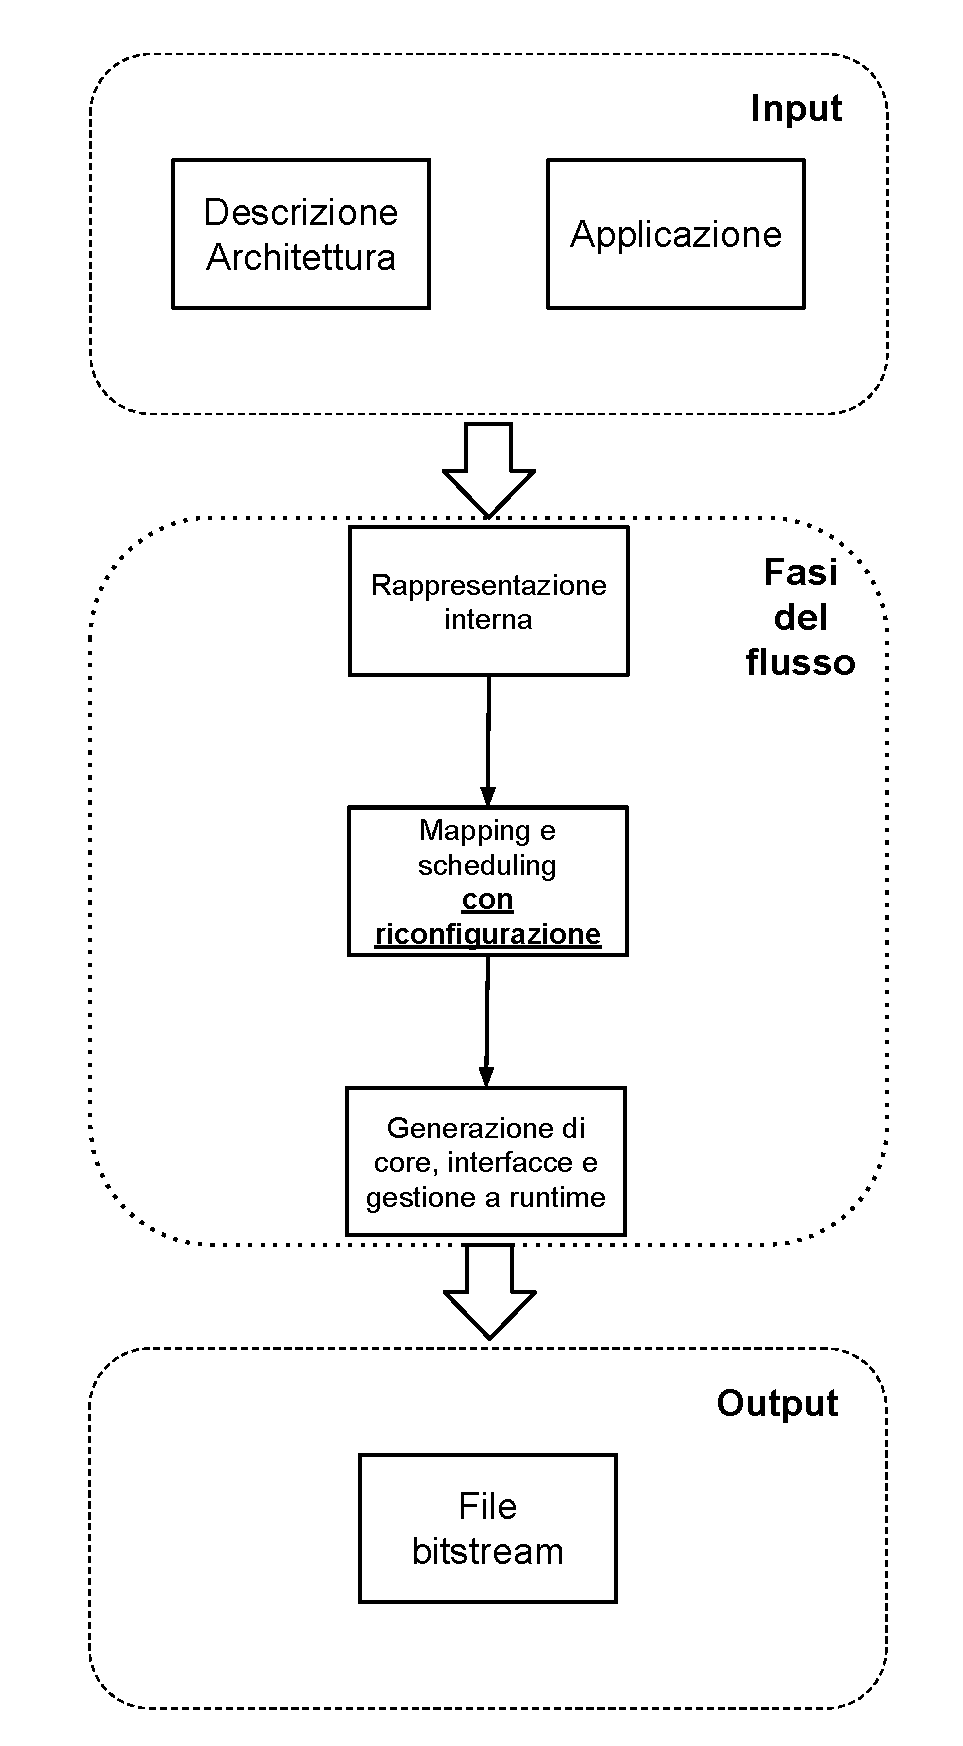
\includegraphics[width=0.6\textwidth]{./capitoli/figure/cap1/StrutturaFlusso.pdf}
    \caption{Struttura di un flusso generico, con input e output.}
    \label{fig:strutturaFlusso}
  \end{center}
\end{figure}

Come rappresentato in figura \ref{fig:strutturaFlusso}, un flusso generico ha come dati di input la descrizione
dell'architettura target e dell'applicazione, scritta in un linguaggio di alto livello;
al termine dell'elaborazione, l'output restituito \`e l'insieme di direttive di configurazione sotto forma
di bitstream, o serie di bitstream. Le fasi del flusso possono essere effettuate manualmente
oppure automatizzate del tutto o in parte. Nei prossimi paragrafi i componenti della struttura verranno descritti
maggiormente nel dettaglio.

\subsubsection{Input}
\begin{enumerate}
  \item \emph{descrizione dell'architettura}: rappresenta, mediante una specifica ad alto livello (ad esempio
    in formato XML), l'architettura target del sistema:
    \begin{itemize}
      \item caratteristiche dei dispositivi riconfigurabili presenti;
      \item caratteristiche dei processori software presenti;
      \item elementi di comunicazione e interconnessioni;
      \item descrizione delle memorie.
    \end{itemize}
  \item \emph{descrizione dell'applicazione}: algoritmi che compongono l'applicazione da implementare sul sistema
    in linguaggio ad alto livello (ad esempio C, C++ o altro).
\end{enumerate}

\subsubsection{Fasi del flusso}
\begin{itemize}
  \item Codifica dell'applicazione nella rappresentazione interna del tool di sviluppo;
  \item \emph{partizionamento HW/SW}, \emph{mapping} e \emph{scheduling};
  \item generazione dei sorgenti software e core hardware;
  \item generazione delle interfacce di comunicazione;
  \item gestione a runtime dell'applicazione.
\end{itemize}
L'applicazione viene dapprima codificata in una
rappresentazione interna al flusso, che ne consente la manipolazione e
l'elaborazione da parte del tool di sviluppo. Esistono diverse possibili
rappresentazioni, nel contesto di questo lavoro ci riferiremo alla
rappresentazione tramite \emph{task graph}, descritta nella sezione
\ref{subsec:modello}. L'applicazione viene quindi suddivisa in un
insieme di task caratterizzati da dipendenze.\footnote{Nel contesto di questo
lavoro, i task sono collegati da relazioni produttore-consumatore; pertanto, un arco $(i,j)$ nel task graph implica che
l'output del task $i$ sia l'input del task $j$.}

Nella fase di \emph{partizionamento HW/SW} viene stabilito quali task verranno
eseguiti in hardware e quali su un processore general-purpose, oltre ad assegnare le risorse computazionali ai vari task in
base al partizionamento calcolato (fase di
\emph{mapping}); in questa fase si effettua anche lo
\emph{scheduling}. Le fasi di mapping e scheduling assumono particolare
importanza nello sviluppo di \ac{MPSoC} riconfigurabili. Durante la fase di mapping,
infatti, possono essere sfruttate le potenzialit\`a offerte dalla riconfigurazione,
per eseguire diverse parti dell'applicazione sulla stessa porzione di logica riconfigurabile.
La possibilit\`a di sfruttare la riconfigurazione fornisce quindi un grado di libert\`a aggiuntivo
al designer, e allo stesso tempo, aumenta la complessit\`a dei problemi di mapping e scheduling.
Queste fasi, oggetto del lavoro, verranno descritte nella prossima sezione.

Dopo il partizionamento delle risorse vengono generati i sorgenti software per
eseguire i task assegnati al processore general-purpose e i core hardware per i
task assegnati a implementazioni hardware dedicate.

A questo punto vengono generate le interfacce di comunicazione utilizzate dai
moduli hardware per comunicare tra loro e interfacciarsi con gli altri
componenti del sistema, ad esempio la memoria; dopo la generazione delle
interfacce vengono creati i driver, che astraggono dal protocollo di
comunicazione utilizzato.

In ultimo, il sistema viene completato generando la gestione a runtime dell'applicazione e i componenti
hardware vengono integrati nel sistema.

\subsubsection{Output}
In uscita del flusso si ha la configurazione del sistema MPSoC, pronta per essere caricata sulla scheda;
il bitstream finale viene solitamente generato utilizzando strumenti proprietari del produttore della scheda.


\section{Definizione del problema}
\label{sec:definizioneProblema}
L'obiettivo di questa sezione \`e descrivere nel dettaglio le fasi di \emph{mapping} e \emph{scheduling}
dei task, introdotte nella precedente sezione, e le problematiche che emergono in questa fase con riferimento
specifico al caso di design di un sistema riconfigurabile.
Mapping e scheduling sono l'oggetto di questo lavoro di tesi, che come obiettivo principale si prefigge di
automatizzare queste fasi, determinando inoltre quando e se utilizzare la riconfigurazione parziale dinamica
sia vantaggioso per l'esecuzione dell'applicazione, considerando diverse possibili metriche per l'ottimizzazione.

La sezione \ref{subsec:modello} fornisce il modello del problema, tramite una formulazione matematica tratta
da \cite{ModelloRedaelli,ReconfigurableSystemDesignVerification}.

La sezione \ref{subsec:mappingScheduling} descrive nel dettaglio le due fasi oggetto del lavoro, evidenziando
la loro forte interdipendenza e i problemi che si devono affrontare nell'effettuare queste fasi.

\begin{figure}[ht]
\begin{center}
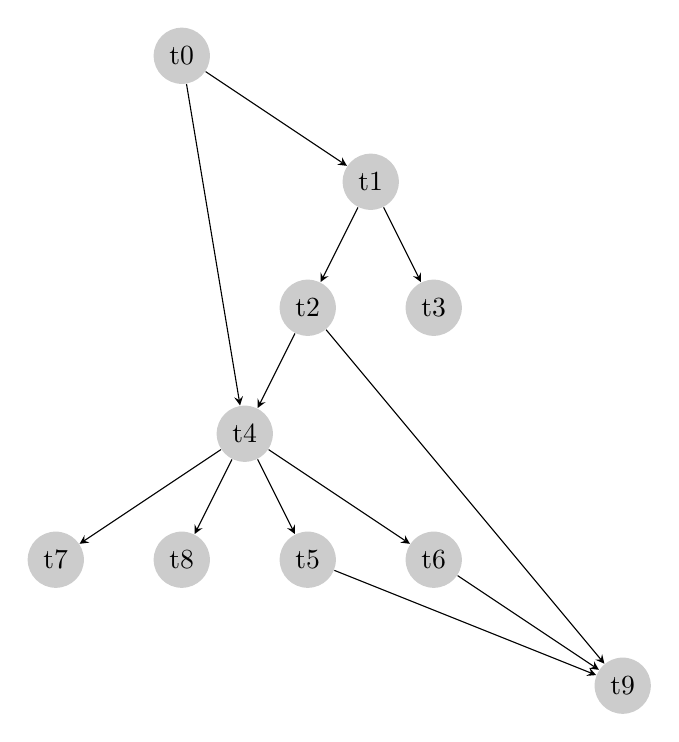
\begin{tikzpicture}[scale=.8,auto=left,every node/.style={circle,fill=gray!40},>=stealth]
 \node (n0) at (1,10) {t0};
 \node (n1) at (4,8) {t1};
 \node (n2) at (3,6) {t2};
 \node (n3) at (5,6) {t3};
 \node (n4) at (2,4) {t4};
 \node (n5) at (3,2) {t5};
 \node (n6) at (5,2) {t6};
 \node (n7) at (-1,2) {t7};
 \node (n8) at (1,2) {t8};
 \node (n9) at (8,0) {t9};
 
 \foreach \from/\to in 
{n0/n1,n0/n4,n1/n2,n1/n3,n2/n4,n4/n7,n4/n8,n4/n5,n4/n6,n2/n9,n6/n9,n5/n9}
\draw [->] (\from) -- (\to);
\end{tikzpicture}
\caption{Esempio di task graph.}
\label{fig:taskGraphExample}
\end{center}
\end{figure}

\subsection{Modello}
\label{subsec:modello}
Come anticipato nella sezione \ref{subsec:introFlussi}, la specifica dell'applicazione
da accelerare è data sotto forma di un grafo che
rappresenta il flusso di esecuzione dell'applicazione, chiamato \emph{task
graph}: questo è composto da \emph{task},
che rappresentano unità computazionali, ed \`e descritto nella forma
$\langle S, P \rangle$, dove $S$ è l'insieme dei task (nodi del grafo) e $P$
\`e l'insieme delle precedenze tra i task (archi del grafo).
In figura~\ref{fig:taskGraphExample} è possibile vedere un esempio di
task graph.

A ogni task corrispondono una o più \emph{implementazioni}, ovvero diversi modi di
realizzarne la funzionalità; le implementazioni possono essere di due tipi: software
oppure hardware. Le prime sono prodotte dai compilatori, ne possono
esistere più versioni per ogni task date da differenti ottimizzazioni abilitate dal
compilatore.
Nel caso delle implementazioni hardware, pu\`o capitare che un particolare task non sia adatto
alla sintesi a causa di particolari costrutti al suo interno; in questo caso si pu\`o modificare
la struttura del task conservandone la semantica, ottenendo un task equivalente e sintetizzabile.
Solitamente, possono esistere più implementazioni hardware per un singolo task,
che differiscono per il tempo di esecuzione e l'area che occupano su scheda.

Sfruttando la notazione tratta da \cite{ModelloRedaelli}
e \cite{ReconfigurableSystemDesignVerification}, il dispositivo riconfigurabile viene 
rappresentato come una griglia di \ac{RU}, costituita da un insieme di righe
$R=\left\{r_1, r_2, \dots, r_{\vert R \vert}\right\}$ e 
di colonne $C=\left\{c_1, c_2, \dots, c_{\vert C \vert}\right\}$. Ogni unità 
riconfigurabile è rappresentata da una tupla $(r,c) \in U$ con $r \in R$ e $c \in C$, e 
composta da un numero $\rho_{u}$ di \ac{CLB}.

Le implementazioni sono realizzate tramite particolari combinazioni di risorse (\ac{RU}),
e vengono definite \ac{EU}. A ogni task può quindi corrispondere una o più \ac{EU}.

\subsubsection{Partizionamento e scheduling}
Data la formulazione precedentemente descritta, è possibile formulare il problema
di partizionamento e scheduling su architetture riconfigurabili come illustrato in questa
sezione. I task devono essere mappati su un insieme $E$ di \acp{EU}, 
ottenute configurando le unità riconfigurabili tramite bitstream che specificano 
l'implementazione di tali task.

Nell'ipotesi di poter calcolare o stimare il tempo di esecuzione $l_{s}$, di 
riconfigurazione $d_{s}$ e l'area occupata $r_{s}$ da un task, si può quindi modellizzare 
la ricerca della soluzione come la definizione di una funzione 
che, dati questi input, specifica per ogni task:
\begin{itemize}
 \item l'\ac{EU} $e_s \in E$ su cui deve essere mappato, e il suo posizionamento 
all'interno dell'\ac{FPGA} in termini di \ac{RU};
 \item il tempo di inizio della riconfigurazione per l'\ac{EU}, $\bar{t}_s \in T$;
 \item il tempo di inizio dell'esecuzione del task $t_s \in T$.
\end{itemize}

In maniera formale:
\begin{equation}
\label{formula:mappingScheduling}
 \sigma : S \rightarrow E \times 2^{U} \times T \times T
\end{equation}

Data la formulazione appena introdotta, le fasi nel design di sistemi riconfigurabili
oggetto di questo lavoro si possono definire nel modo seguente:
\begin{enumerate}
 \item \emph{partitioning}: in questa fase viene stabilito quali task devono essere
 eseguiti in software e quali in hardware;
 \item \emph{mapping}: decisione della particolare implementazione e \emph{processing
 element}\footnote{Il concetto di processing element è simile a quello di combinazione
 di \ac{RU}; tuttavia, mentre una combinazione di \ac{RU} rappresenta solo una generica
 area su logica riconfigurabile, il termine ``processing element`` racchiude anche unità
 di computazione non riconfigurabili, come core implementati staticamente su scheda oppure
 microprocessori.}
 con cui realizzare la funzionalità di ogni task;
 \item \emph{scheduling}: assegnazione dei tempi di inizio/fine esecuzione dei task,
 rispettando le precedenze;
\end{enumerate}
Il lavoro descritto in questa tesi si concentra su una possibile soluzione per il 
problema di mapping\footnote{Nel contesto di questo lavoro, il termine \emph{mapping}
comprende anche la fase di partizionamento.} e scheduling dei task.


\subsection{Le fasi di mapping e scheduling}
\label{subsec:mappingScheduling}
La fase di mapping ha il
compito di determinare dove i task dell'applicazione debbano essere eseguiti
(su quale processing element) e in quale modo (con quale tra le possibili implementazioni).

Il compito dello scheduler è invece assegnare i tempi di inizio e di fine dell'esecuzione ai
task che compongono l'applicazione.


\subsubsection{Obiettivi di mapping e scheduling}
Dato un numero sufficiente di processing element, siano essi hardware o software, un generico
task graph ammette diversi possibili schedule che ne rispettino le 
precedenze, per ogni possibile mapping. Sfortunatamente, non tutte le scelte di mapping e scheduling
che soddisfano i vincoli di precedenza senza violarne altri (ad esempio, senza eccedere l'area a disposizione
nel caso di implementazioni su hardware riconfigurabile)
hanno uguale ``desiderabilità'' dal punto di vista della soluzione finale. Quindi, una buona fase
di mapping e scheduling deve scegliere gli assegnamenti ottimi o subottimali dal punto di vista di
varie metriche, che sono oggetto dell'ottimizzazione, tra le più importanti si ricordano:
\begin{itemize}
 \item \emph{makespan}: minimizzare la durata totale dell'esecuzione dello schedule, dato un mapping;
 \item \emph{power consumption}: limitare il consumo di energia richiesto 
    dall'esecuzione dei task;
  \item \emph{area usage}: limitare la quantit\`a di risorse hardware richieste,
    tramite assegnamenti di mapping pi\`u conservativi.
\end{itemize}


\subsubsection{Impatto di comunicazioni e riconfigurazioni sullo schedule}
Dato un task graph come quello in figura~\ref{fig:taskGraphExample},
le precedenze esplicitano relazioni produttore-consumatore;
un arco orientato $(i,j)$ simboleggia un trasferimento dell'output della
computazione del task $i$ in memoria (locale o condivisa), per essere utilizzato
successivamente come input per il task $j$.
Gli archi introducono quindi delle
comunicazioni che devono necessariamente essere prese in considerazione nella fase 
di scheduling, poich\'e gli effetti dei trasferimenti di dati sono un aspetto
di cruciale importanza nel determinare correttamente il makespan dell'applicazione \cite{AntColonyOptimization}.

Oltre alle comunicazioni, lo scheduler deve anche gestire il verificarsi di 
riconfigurazioni nel corso dell'esecuzione dell'applicazione. Ad esempio, se due task $i$ 
e $j$ durante la fase di mapping vengono assegnati a uno stesso processing element su 
scheda con due implementazioni diverse, è necessario riconfigurare quella porzione di 
scheda nell'intervallo di tempo che intercorre tra l'esecuzione di $i$ e quella di $j$.
Come visto nella sezione \ref{subsec:introFlussi}, l'overhead introdotto dalle riconfigurazioni
non \`e trascurabile, e pu\`o penalizzare notevolmente il makespan dello schedule.
Un buon algoritmo di scheduling deve pertanto cercare di ``mascherare'' quanto possibile le
riconfigurazioni che devono essere eventualmente fatte. Questa tecnica verr\`a spiegata nel capitolo
\ref{chap:SOA}.

\subsubsection{Complessità}
Come evidenziato dalla formula \eqref{formula:mappingScheduling}, lo spazio di ricerca è 
estremamente ampio, e la complessità delle fasi di mapping e scheduling se effettuate 
contemporaneamente rende quasi impossibile risolvere (in maniera ottima) problemi non 
banali.

Il problema di fissare un mapping e uno schedule per i task di un'applicazione
tale da minimizzare una determinata metrica, o un insieme di metriche nel caso
di ottimizzazione multi-obiettivo) è un classico esempio di \ac{RCSP}; tale
problema appartiene alla classe di complessità computazionale dei problemi
$\mathcal{NP}$-difficili;\footnote{Un problema \`e $\mathcal{NP}$-difficile se la sua \emph{versione
di riconoscimento} \`e $\mathcal{NP}$-completa. Il primo problema ad essere dimostrato
$\mathcal{NP}$-completo \`e il problema di soddisfacibilit\`a booleana \cite{CookSAT}.} per questo tipo di problemi non si è ancora
trovato un algoritmo \emph{esatto} che riesca a risolvere questo problema in
tempo polinomiale, e si pensa che non ne esistano.\footnote{Se esistesse,
varrebbe l'equivalenza $\mathcal{P} = \mathcal{NP}$. Questa congettura, non ancora
dimostrata, \`e uno dei principali problemi non ancora risolti della teoria sulla
complessit\`a computazionale \cite{GasarchPoll}.}

Oltre a questo, un'altra difficoltà che si incontra è che il problema dello
scheduling dei task non è indipendente dalla fase di partitioning/mapping; le
due fasi sono strettamente collegate e devono essere risolte contemporaneamente
per garantire il raggiungimento degli obiettivi ottimali
\cite{AntColonyOptimization}. Tuttavia, ciò aumenta ulteriormente la
complessità del problema e lo spazio delle possibili soluzioni.


\subsubsection{Algoritmi utilizzabili} Esistono diversi algoritmi per risolvere
il problema di mapping e scheduling dei task, alcuni esatti basati sulla
\ac{PLI}, altri basati su euristiche più o meno complesse che ricercano
soluzioni sub-ottime, entrambi i tipi saranno discussi più nel dettaglio nel
capitolo~\ref{chap:SOA}, in particolare nella
sezione~\ref{sec:algoritmiProposti}.  Lo svantaggio a livello pratico degli
algoritmi esatti è l'eccessivo tempo impiegato per trovare una soluzione nel caso di
applicazioni non banali, limitazione che tende a far preferire l'uso di metodi
non esatti, ma più veloci quali le euristiche, per ottenere risultati buoni in
tempi accettabili; in questo lavoro gli algoritmi proposti per le fasi di
mapping e scheduling sono di tipo euristico, le motivazioni per questa scelta verranno
illustrate nel capitolo~\ref{chap:approccio}.

% TODO outline tesi
